
\subsection{フィボナッチヒープ}
\frame{
  \frametitle{フィボナッチヒープ}
  \begin{block}{Fibonacci Heap}
    全順序集合$P(C,\leq)$について,$C$上からなる要素のフィボナッチヒープは\\
    以下の操作が実行できる
    \itemize{
    \item top : $O(1)$でヒープの最大値を求める
    \item merge : $O(1)$で2つのヒープを併合する
    \item push : $O(1)$で$C$の要素$x$を追加する
    \item pop : $O(\log N)$でヒープの最大値をもつ要素を削除する
    \item size : $O(1)$でヒープの要素数を求める\\
    }
    いいね
  \end{block}
}

\frame{
  \frametitle{フィボナッチヒープ}
  \begin{block}{Fibonacci Heap}
    ヒープ条件を満たす木の集合\\
    2分ヒープや2項ヒープよりも条件が弱い
  \end{block}
  \begin{exampleblock}{例}
    \center{
      \includegraphics<1>[width=10cm]{image/fibonacci01.pdf}
      \includegraphics<2>[width=10cm]{image/fibonacci02.pdf}
      \includegraphics<3>[width=10cm]{image/fibonacci03.pdf}
    }
  \end{exampleblock}
}

\frame{
  \frametitle{push}
  \begin{block}{push$(H, k)$}
    1.  $k$を値に持つ接点$x$を作る\\
    2.  insert$(head[H], x)$\\
    3.  {\bf If} $k > key[head[H]]$\\
    4. ~~ {\bf Then} $head[H] \leftarrow right[head[H]]$
  \end{block}
}

\frame{
  \frametitle{push}
  \begin{block}{push}
    根リストに接点を挿入する
  \end{block}
  \begin{exampleblock}{例}
    \center{
      \includegraphics<1>[width=10cm]{image/fibonacci04.pdf}
      \includegraphics<2>[width=10cm]{image/fibonacci05.pdf}
    }
  \end{exampleblock}
}

\frame{
  \frametitle{merge}
  \begin{block}{merge$(H, H')$}
    1.  $left[right[head[H]]] \leftrightarrow left[right[head[H']]]$\\
    2.  $right[head[H]] \leftrightarrow right[head[H]]$\\
    3.  {\bf If} $key[head[H']] > key[head[H]]$\\
    4. ~~ {\bf Then} $head[H] \leftarrow head[H']$
  \end{block}
}

\frame{
  \frametitle{merge}
  \begin{block}{merge}
    2つの根リストを結合する
  \end{block}
  \begin{exampleblock}{例}
    \center{
      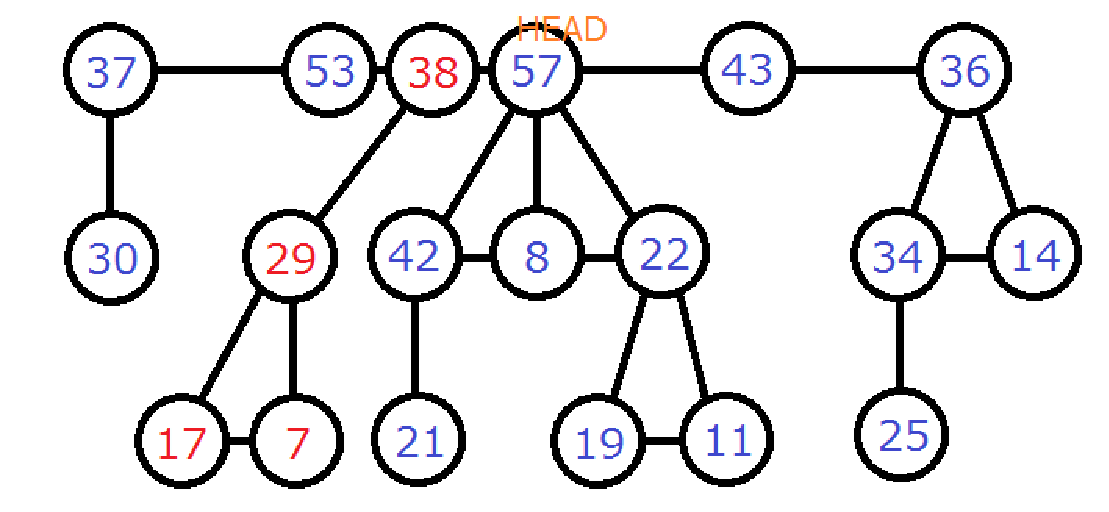
\includegraphics[width=10cm]{image/fibonacci06.pdf}
    }
  \end{exampleblock}
}

\frame{
  \frametitle{pop}
  \begin{block}{pop$(H)$}
    1.  $head[H]$を$H$の根リストから削除する\\
    2.  $head[H]$の子を全て根リストに追加する\\
    3.  $head[H] \leftarrow child[head[H]]$\\
    4.  根リストに含まれる全ての接点の次数が異なるように整理する\\
    5.  根リストから最大値を持つ接点を探し,それをheadにする
  \end{block}
}

\frame{
  \frametitle{pop}
  \begin{exampleblock}{例}
    \center{
      \includegraphics<1>[width=10cm]{image/fibonacci07.pdf}
      \includegraphics<2>[width=10cm]{image/fibonacci08.pdf}
      \includegraphics<3>[width=10cm]{image/fibonacci09.pdf}
      \includegraphics<4>[width=10cm]{image/fibonacci10.pdf}
      \includegraphics<5>[width=10cm]{image/fibonacci11.pdf}
      \includegraphics<6>[width=10cm]{image/fibonacci13.pdf}
      \includegraphics<7>[width=10cm]{image/fibonacci13.pdf}
      \includegraphics<8>[width=10cm]{image/fibonacci14.pdf}
      \includegraphics<9>[width=10cm]{image/fibonacci15.pdf}
      \includegraphics<10>[width=10cm]{image/fibonacci16.pdf}
      \includegraphics<11>[width=10cm]{image/fibonacci17.pdf}
      \includegraphics<12>[width=10cm]{image/fibonacci18.pdf}
    }
  \end{exampleblock}
}

%\subsection{AVL木}
%\subsection{Union-Find Tree}
%\subsection{Segment Tree}
%\subsection{Fenwick Tree}
%\subsection{Wavelet Tree}
